\documentclass[conference,a4paper]{IEEEtran}
\IEEEoverridecommandlockouts
\usepackage[left=1.57cm,right=1.57cm,top=0.95cm,bottom=2.54cm]{geometry}
\newpage % Mulai halaman kedua
% \usepackage{caption}

% \captionsetup[figure]{justification=raggedright, singlelinecheck=off}

% Mengubah margin pada halaman kedua
\newgeometry{left=1.57cm,right=1.57cm,top=1.9cm,bottom=2.54cm}
% The preceding line is only needed to identify funding in the first footnote. If that is unneeded, please comment it out.
\usepackage{cite}
\usepackage{amsmath,amssymb,amsfonts}
\usepackage{algorithmic}
\usepackage{graphicx}
\usepackage{textcomp}
\usepackage{xcolor}
\usepackage{balance}
\usepackage{multirow}
\def\BibTeX{{\rm B\kern-.05em{\sc i\kern-.025em b}\kern-.08em
    T\kern-.1667em\lower.7ex\hbox{E}\kern-.125emX}}
\begin{document}

\title{
  Advancing Statistical Education with RWikiStat 4.0: A Comprehensive Multi-Platform Learning Application
  \\
  \thanks{*Corresponding Author}
}

\makeatletter
\newcommand{\linebreakand}{
  \end{@IEEEauthorhalign}
  \hfill\mbox{}\par
  \mbox{}\hfill\begin{@IEEEauthorhalign}
}
\makeatother

\author{
  \IEEEauthorblockN{Hizir Sofyan}
  \IEEEauthorblockA{\textit{Statistics Department} \\
    \textit{Universitas Syiah Kuala}\\
    Banda Aceh, Indonesia 23111\\
    hizir@usk.ac.id}
  \and
  \IEEEauthorblockN{Munawar}
  \IEEEauthorblockA{\textit{Statistics Department} \\
    \textit{Universitas Syiah Kuala}\\
    Banda Aceh, Indonesia 23111 \\
    munawar@mhs.usk.ac.id}
  \and
  \IEEEauthorblockN{Muhammad Subianto}
  \IEEEauthorblockA{\textit{Informatics Department} \\
    \textit{Universitas Syiah Kuala}\\
    Banda Aceh, Indonesia 23111\\
    subianto@usk.ac.id}
  \and
  \IEEEauthorblockN{Kurnia Saputra\textsuperscript{*}}
  \IEEEauthorblockA{\textit{Informatics Department} \\
    \textit{Universitas Syiah Kuala}\\
    Banda Aceh, Indonesia 23111\\
    kurnia.saputra@usk.ac.id}
  \and
  \linebreakand
  \IEEEauthorblockN{Naufal Mas Adha}
  \IEEEauthorblockA{\textit{Informatics Department} \\
    \textit{Universitas Syiah Kuala}\\
    Banda Aceh, Indonesia 23111\\
    naufal@mhs.usk.ac.id}
  \and
  \IEEEauthorblockN{Affan Ian Amara}
  \IEEEauthorblockA{\textit{Informatics Department} \\
    \textit{Universitas Syiah Kuala}\\
    Banda Aceh, Indonesia 23111\\
    affan@mhs.usk.ac.id}
  \and
  \IEEEauthorblockN{Muhammad Nurifai}
  \IEEEauthorblockA{\textit{Informatics Department} \\
    \textit{Universitas Syiah Kuala}\\
    Banda Aceh, Indonesia 23111\\
    nurifai@mhs.usk.ac.id}
  \and
  \IEEEauthorblockN{Akhyar}
  \IEEEauthorblockA{\textit{Informatics Department} \\
    \textit{Universitas Syiah Kuala}\\
    Banda Aceh, Indonesia 23111\\
    akhULFA1@mhs.usk.ac.id}
}

\maketitle

\begin{abstract}
  RWikiStat 4.0 is a multi-platform learning application designed to enhance the teaching and learning experience in statistical education. Building on the strengths of its predecessors, RWikiStat 4.0 addresses the limitations of accessibility, interactivity, and collaboration by introducing features such as Shiny-based interactive data visualization, discussion forums, AI-powered chatbots, and R language compilers. Developed for web, Android, and iOS platforms, this version ensures cross-device compatibility and improved user experience. Testing results demonstrate high usability and user satisfaction, highlighting its potential as a comprehensive and innovative tool for statistical education. This application empowers students and educators to engage in dynamic, flexible, and interactive learning, setting a new standard in the field of statistical education.
\end{abstract}

\begin{IEEEkeywords}
  RWikiStat 4.0, Statistical Education, Multi-Platform Learning, Shiny Visualization, Interactive Learning, AI Chatbot, Cross-Device Compatibility, R Language Compiler.
\end{IEEEkeywords}

\section{Introduction}
\label{sect:introduction}

Statistics is a compulsory subject that many students consider difficult.
Especially if the teaching method provided is too rigid and uninteresting. In
recent decades, research in statistical learning has changed the structure of
learning, namely by considering innovative pedagogical instruction, educational
technology, and abundant Web resources \cite{b1}. In the GAISE guidelines, it
is recommended that statistics teaching focus on projects, lab exercises, and
group discussions rather than traditional lectures to improve students'
understanding of the material \cite{b2}. One statistical learning system that
implements this is RWikiStat.

Rwikistat is an example of a digital learning system that has had a positive
impact in the field of education. This application has been developed in 3
versions, namely in 2010, 2012, and 2019. RWikiStat was initially developed in
the form of a website in 2010 with the name Rweb to support users in inserting
compiled R code to produce graphic or numerical output. Then, after being
integrated with the wiki application, this application was finally known as
RWIKISTAT \cite{b3}. The second version of RWikiStat was developed on the Linux
operating system and is open source. In this version, users can edit web
content, access it offline without requiring prior installation, as well as
develop Live DVDs to ensure the application remains safe \cite{b4}. In 2019,
RWikiStat 3.0 was developed as an Android application with a more responsive
and easy-to-use interface \cite{b5}.

Although each version has made a significant contribution to the learning of
statistics, there are still several aspects that can be improved. First,
application accessibility in previous versions was only available on the web
and Android platforms. This hinders the flexibility of users who need
cross-device applications, including iOS. Furthermore, this application does
not yet integrate features such as Shiny to visualize data in an attractive way
for users. Third, real time collaboration features and discussion forums are
not yet available so learning is less dynamic. Lastly, there is no adaptive
support, such as AI-based assistance to answer questions from users.

To overcome these problems, this research aims to develop version 4.0 of the
RWikiStat application to optimize previous versions. RWikiStat 4.0 was
developed in a multi-platform form in the form of a website and mobile on the
Android and iOS platforms with a more attractive appearance and has the
function of presenting statistical theories from basic to advanced levels.
RWikiStat 4.0 has several features, including features such as providing a
statistics learning module, a compiler for the R language, discussion forums
and chatbot features, as well as interactive graphic presentations with Shiny.
The shiny package provides a collection of user interface (UI) functions that
have been carefully selected and designed to generate the HTML, CSS, and
JavaScript code required in commands. This step is expected to resolve problems
existing in previous versions to improve user experience on various platforms.

\section{Related Work}
\label{sect:related_work}

This research is a continuation of the development of the statistics learning
application, RWikiStat, which was previously developed to version 3.0. The
first version of RWikiStat was developed in 2010 under the name RWeb in the
form of a website-based application. RWeb initially only focused on solving
statistical problems using R alone to produce graphical or numerical output,
then changed to RWikiStat after being integrated with wiki technology
\cite{b3}. In 2012, this application was developed with the same function but
on the Linux operating system using Live CD/DVD \cite{b4}. Both versions have
several drawbacks such as a complicated interface, inefficient features, and
lack of mobility. The next version of RWikiStat was developed as an Android
application with a more responsive and easy-to-use interface \cite{b5}.
However, these three versions still require improvement because they still have
several shortcomings, such as still using Rweb (web interface for R statistical
software) and Wiki media. Not yet using more modern interactive media.

One interactive media that can be used is Shiny. Shiny is a package in the R
programming language that allows users to easily create rich and interactive
website-based applications \cite{b6}. The Shiny package offers a variety of
user interface (UI) functions that are carefully designed to generate the HTML,
CSS, and JavaScript code needed in a command. In 2017, six Shiny web
applications were developed for students in introductory statistics or data
analysis classes at Humboldt-Universität zu Berlin. These applications cover
topics such as cluster analysis, regression, and data visualization, and
demonstrate technical implementation and iterative improvements. Evaluation of
an application's usability plays an important role in its development, and
future additions and improvements are also discussed \cite{b7}. Shiny was also
integrated into research developed by Satyahadewi et al. This research
succeeded in developing a web-based application using Shiny for inferential
statistics, showing that this framework is effective in supporting the
development of statistical learning applications \cite{b9}. Research conducted
by González et al. also successfully integrated Shiny to facilitate students'
exploration of statistical concepts through an interactive interface \cite{b9}.

\section{Design and Implementation}
\label{sect:d_and_i}

\subsection{System Architecture}
RWikiStat 4.0 is designed with a multi-platform architecture that allows access
across a variety of devices, including web, Android, and iOS. For mobile
application development, Expo React Native is used, while the web version uses
Next.js as the frontend framework. Both platforms, both mobile and web, share
the same backend, which was developed using Express to ensure data consistency
and server management efficiency.

This application is built with a client-server architecture, where the client
side, both on the web and mobile platforms, is responsible for handling user
interaction and data presentation. The server side developed using Express is
responsible for heavy tasks, such as statistical analysis and data processing,
with extensive R library support. This architecture ensures applications are
modular, scalable, and easy to maintain, and allows for consistent updates
across all platforms.

\subsection{User Interface and User Experience Design}
The UI/UX design in RWikiStat 4.0 focuses on improving experiences that are
attractive and easy to understand for users, both on web and mobile platforms.
The web version is built with a clean and responsive layout that adapts to
various screen sizes. Meanwhile, the mobile version provides a similar
experience with adjustments to the interface and touch interactions for Android
and iOS devices. Users can easily access the features provided on various
platforms. An application interface that prioritizes ease of use, grouping each
component logically and with clear navigation. An easy-to-understand navigation
system allows users to quickly access key features.

The following is a interface of the RWikiStat 4.0 application interface on
various platforms, which illustrates the implementation of the design in the
web and mobile versions:

\begin{figure}[htb]
  \centering
  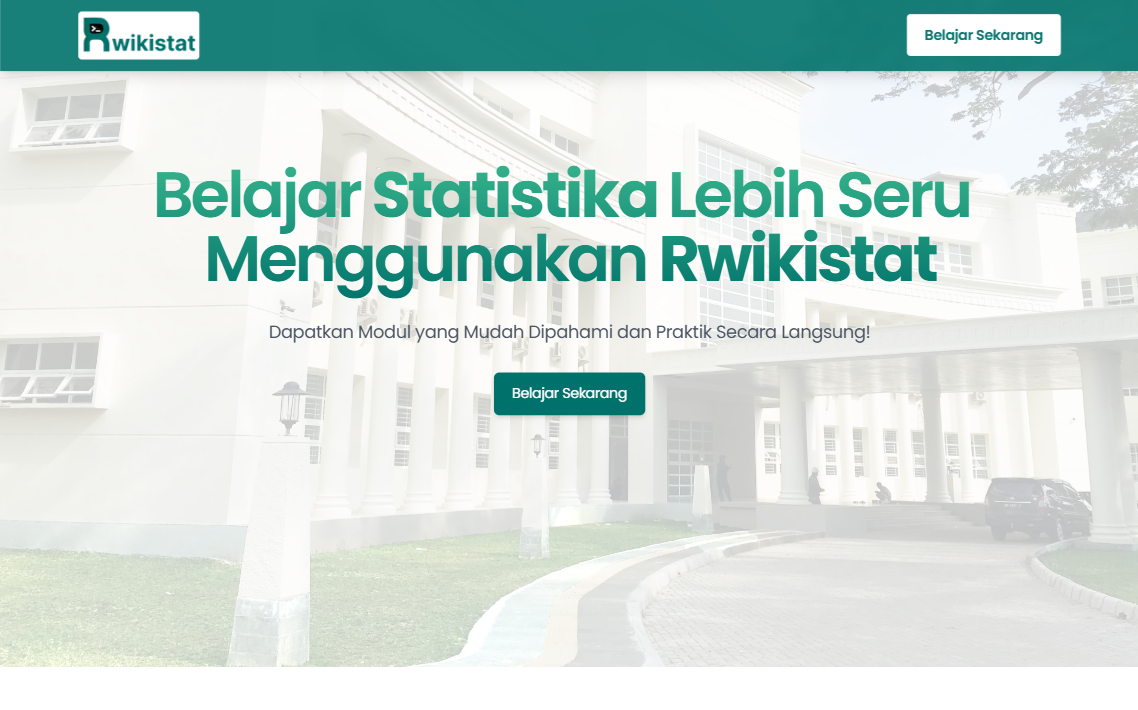
\includegraphics [width=8.5 cm, height=6 cm]{images/web-welcome}
  \caption{Web Welcome Screen}
  \label{distribution}
\end{figure}

\begin{figure}[htb]
  \centering
  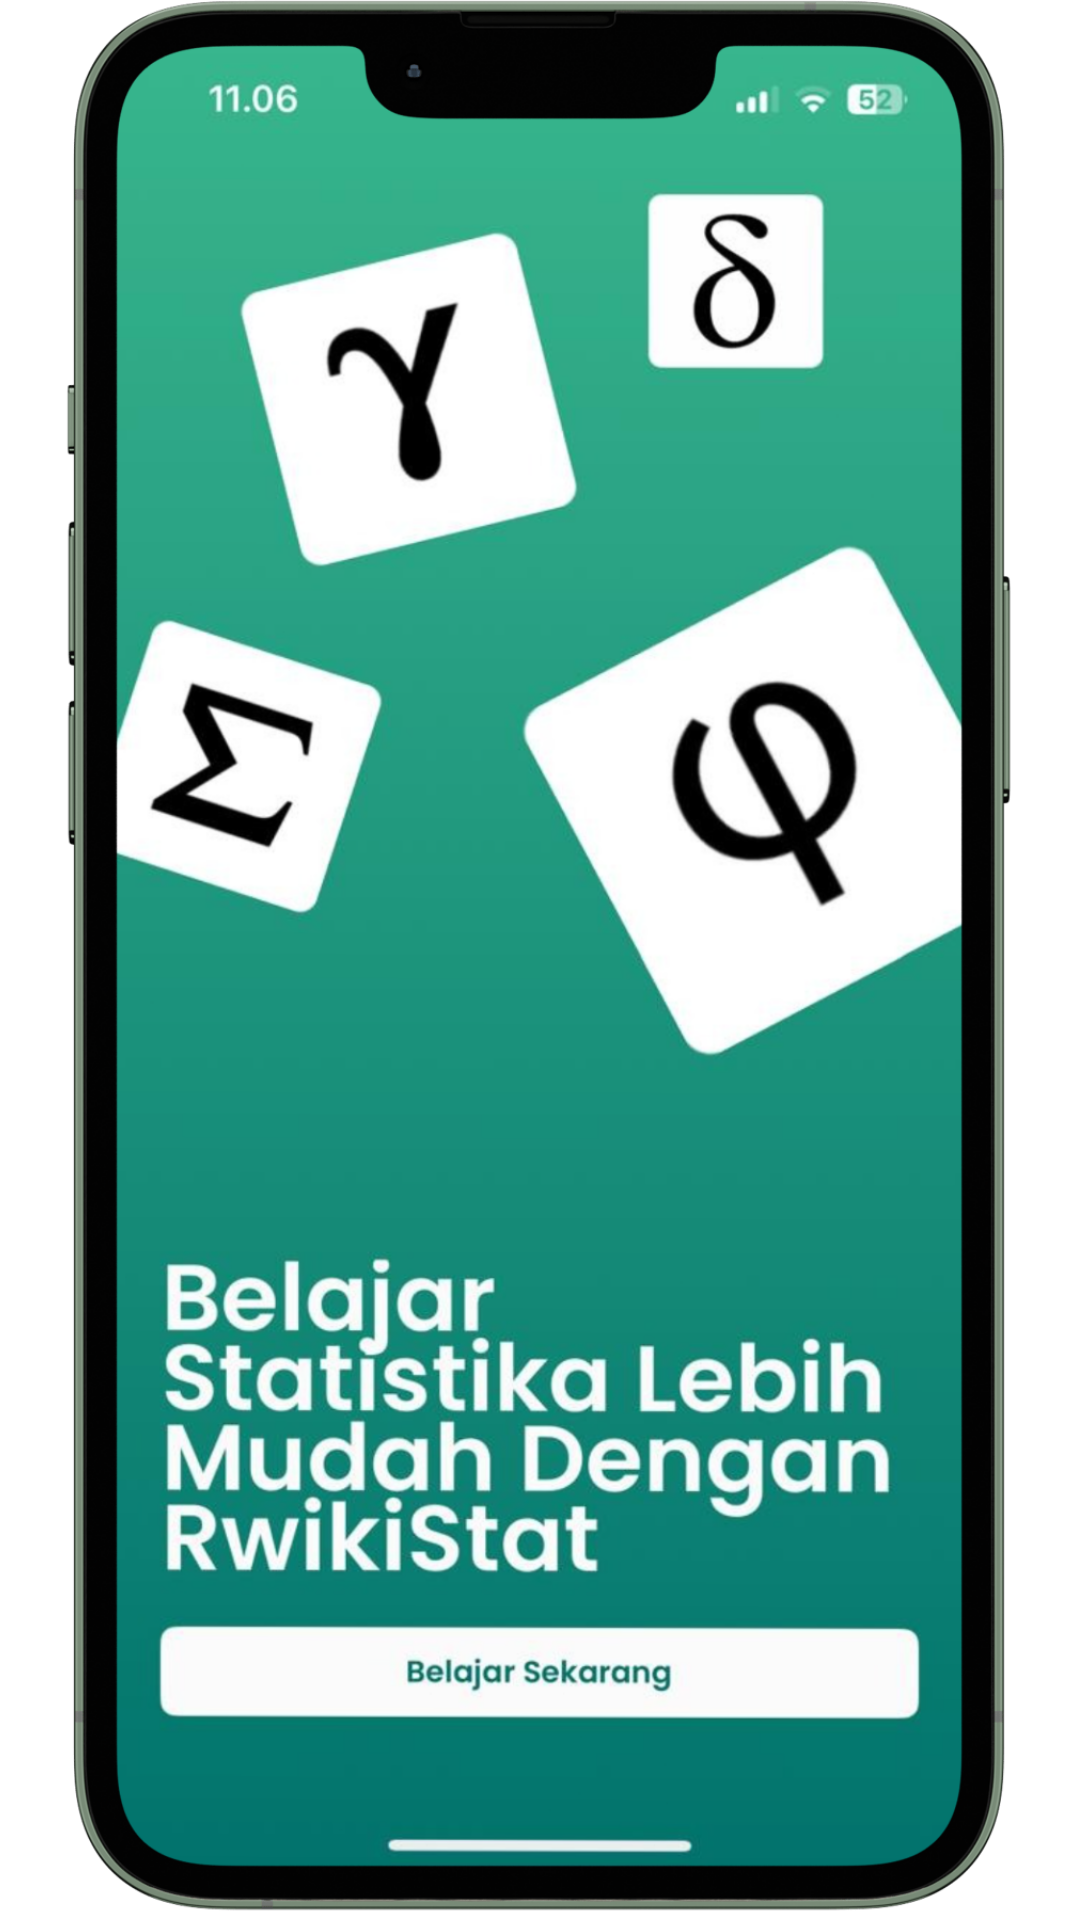
\includegraphics [width=4 cm, height=8 cm]{images/welcome}
  \caption{Mobile Welcome Screen}
  \label{distribution}
\end{figure}

% \begin{figure}[htb]
%   \centering
%   \fbox{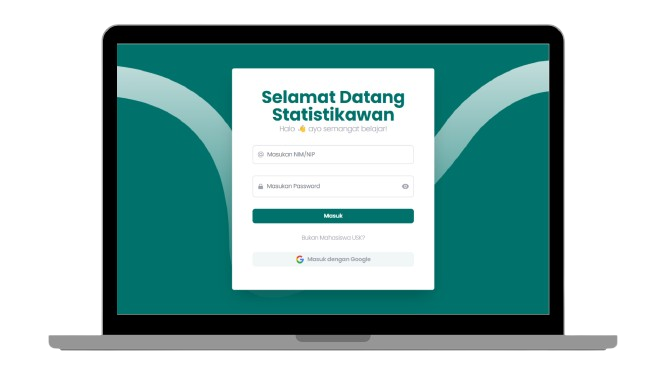
\includegraphics [width=8.5 cm, height=6 cm]{images/web-login}}
%   \caption{Web Login Screen}
%   \label{distribution}
% \end{figure}

% \begin{figure}[htb]
%   \centering
%   \fbox{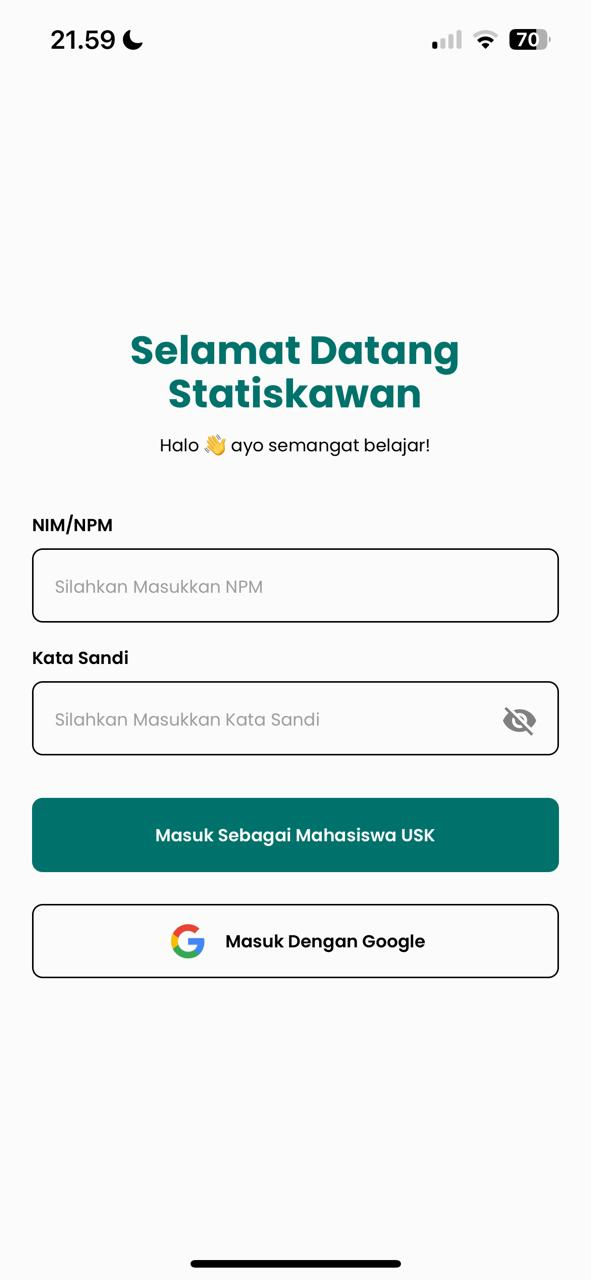
\includegraphics[width=4cm, height=8cm]{images/login}}
%   \caption{Mobile Login Screen}
%   \label{distribution}
% \end{figure}

% \begin{figure}[htb]
%   \centering
%   \fbox{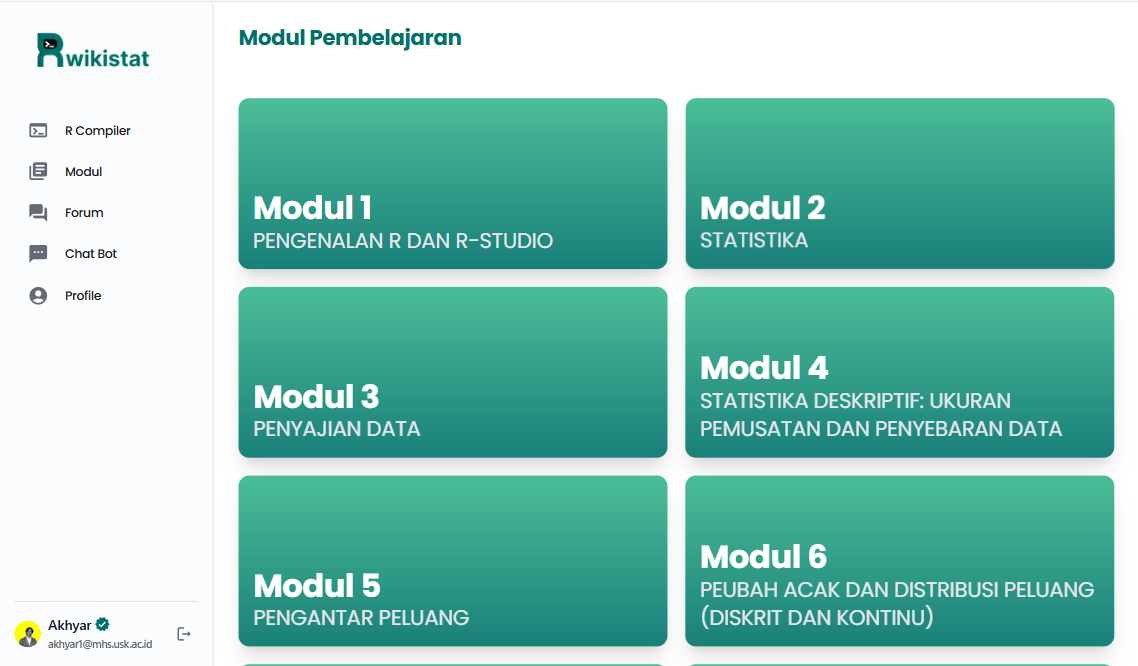
\includegraphics [width=8.5 cm, height=6 cm]{images/web-modul}}
%   \caption{Web Materials Screen}
%   \label{distribution}
% \end{figure}

% \begin{figure}[htb]
%   \centering
%   \fbox{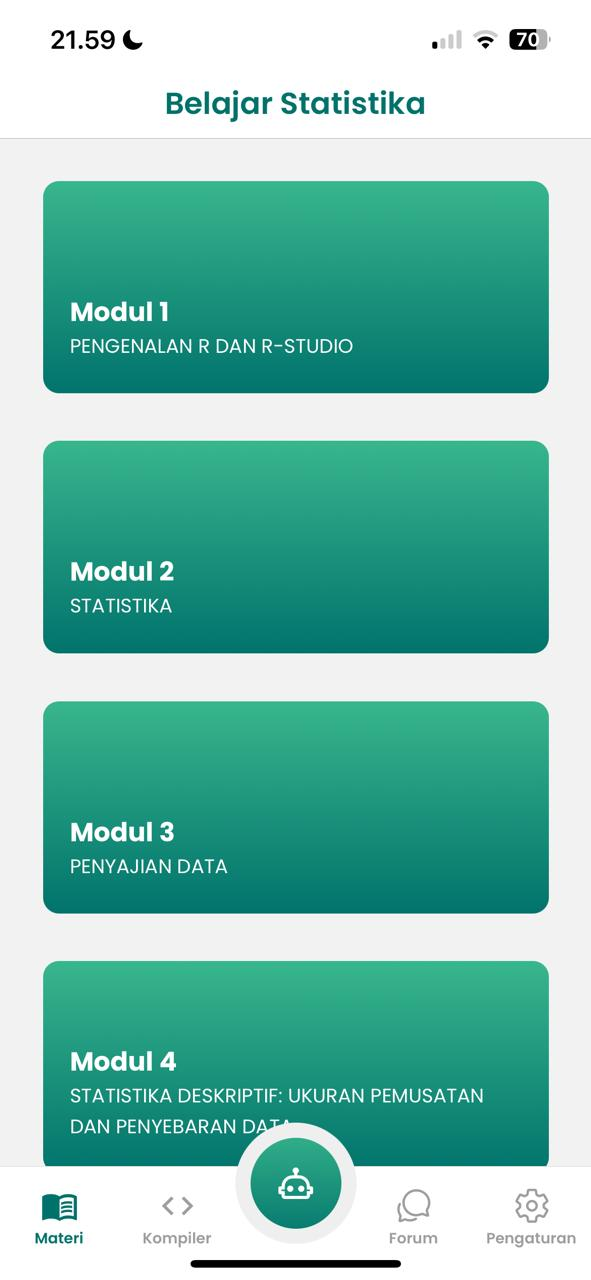
\includegraphics[width=4cm, height=8cm]{images/home}}
%   \caption{Mobile Materials Screen}
%   \label{distribution}
% \end{figure}

% \begin{figure}[htb]
%   \centering
%   \fbox{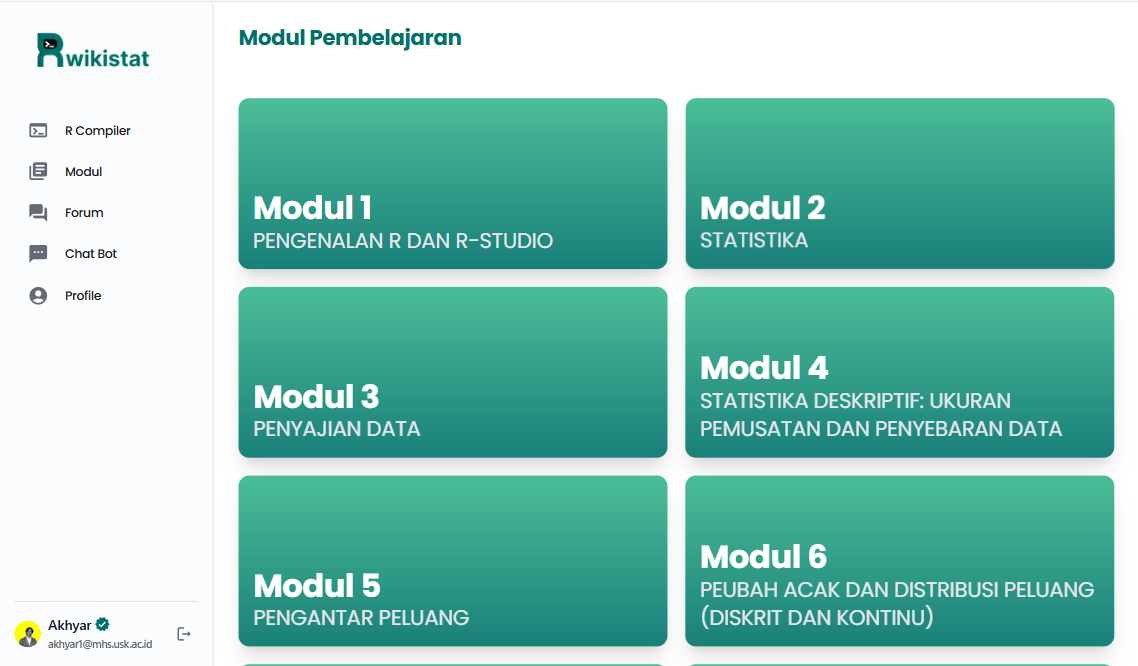
\includegraphics [width=8.5 cm, height=6 cm]{images/web-modul}}
%   \caption{Login Screen Web}
%   \label{distribution}
% \end{figure}

% \begin{figure}[htb]
%   \centering
%   \fbox{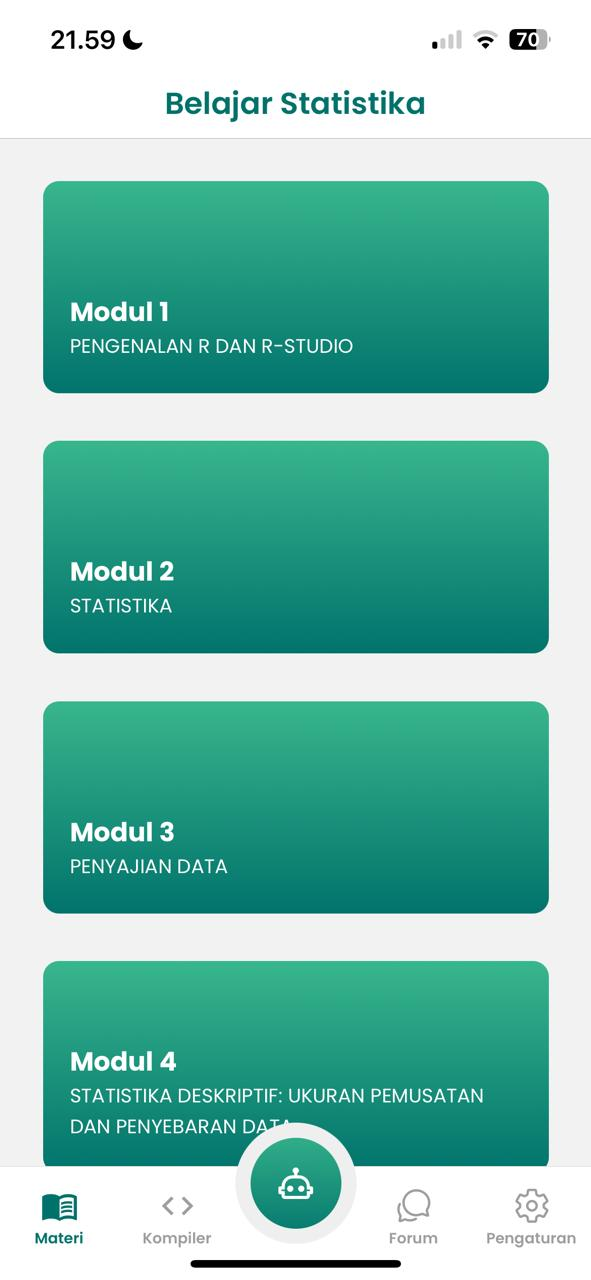
\includegraphics[width=4cm, height=8cm]{images/home}}
%   \caption{Login Screen Mobile}
%   \label{distribution}
% \end{figure}

\subsection{Main Features}
RWikiStat 4.0 develops several new features to enhance the statistics learning
experience for users. One of its main features is the use of Shiny to visualize
data in an attractive and interactive way. This visualization includes common
statistical diagrams, such as histograms, scatter diagrams, and box plots,
which can be customized based on user preferences. With this feature, users can
understand the data more deeply, because of the visualizations displayed. This
also helps users understand complex statistical concepts through direct
interaction.

The next important feature is the discussion forum, which supports dynamic
learning. This feature allows users to engage in discussions, ask and answer
questions, and share insights related to statistical problems to the forum.
With this feature available on all platforms, users can choose to discuss
through the desired device. Another important feature is the sample code for
each learning module. In addition to improving user understanding of the
material, this feature also makes learning more interesting. Users can
immediately try the examples and exercises provided in the module.

In this version, there is also an AI-based chatbot feature that can provide
guidance in understanding statistical concepts to users. Users can ask various
questions about statistics, such as data analysis, functions in R, and various
theories about methods in statistics. With the chatbot feature, users will get
direct help without having to leave the application to search first. This makes
the learning experience more efficient and enjoyable.

\section{Results and Discussion}
\label{sect:results_discussion}

The RWikiStat application provides a satisfactory impact for both web and
mobile versions. This is proven by the results of tests that have been carried
out previously. Testing was carried out using the black box testing method and
the Usability Matrix for User Experience (UMUX). The app runs smoothly, with
fast response times and easy-to-access interactions, both on web and mobile
devices. Test results using black box testing can be seen in table
\ref{tab:testing_results} below

\begin{table}[htbp]
  \caption{BLACKBOX TESTING RESULTS}
  \label{tab:testing_results}
  \renewcommand{\arraystretch}{1.5} % Menambah jarak antar baris
  \resizebox{\columnwidth}{!}{%
    \begin{tabular}{|c|l|l|l|l|}
      \hline
      \textbf{No.} & \textbf{Testing Name}              & \textbf{Scenario}                                                                     & \textbf{Display}                                          & \textbf{Result} \\ \hline
      1            & Sign-in with student ID            & Enter student ID and password in the text input, then press the login button          & Redirected to the main page                               & Success         \\ \hline
      2            & Sign-in with Google                & Press the 'Sign in with Google' button and select a Google account for login          & Redirected to the main page                               & Success         \\ \hline
      3            & Select learning module             & Select one of the module cards                                                        & Redirected to a page containing the module and R compiler & Success         \\ \hline
      4            & Execute R / Shiny code in compiler & Enter simple R / Shiny code to execute                                                & Compilation results of the R code appear                  & Success         \\ \hline
      5            & Add new question in forum          & Fill in the topic title, description, and photo, then press the 'Add Question' button & A new question is added                                   & Success         \\ \hline
      6            & Access learning materials          & Click the materials icon                                                              & The main module page appears                              & Success         \\ \hline
      7            & Access compiler feature            & Click the compiler icon                                                               & The main compiler page appears                            & Success         \\ \hline
      8            & Access forum feature               & Click the forum icon                                                                  & The main forum page appears                               & Success         \\ \hline
      9            & Access profile settings            & Click the settings icon                                                               & The main settings page appears                            & Success         \\ \hline
      10           & Log out of the app                 & Click the logout icon on the settings page                                            & User is redirected to the sign-in page                    & Success         \\ \hline
    \end{tabular}%
  }
\end{table}

In the table \ref{tab:testing_results} can be seen that all test results were
successful, starting from logging in, trying various available features, to
logging out again. Then testing using the UMUX method can be seen in table
\ref{tab:user_feedback} and \ref{tab:umux_results} below

% Please add the following required packages to your document preamble:
% \usepackage{multirow}
% \usepackage{graphicx}
\begin{table}[htbp]
  \caption{UMUX QUESTION LIST \cite{b10}}
  \label{tab:user_feedback}
  \resizebox{\columnwidth}{!}{%
    \begin{tabular}{|c|l|c|}
      \hline
      \textbf{No.} & \textbf{Question}                                      & \textbf{Score} \\ \hline
      1            & This application suits my needs.                       & 1 – 7          \\ \hline
      2            & I had a bad experience using this application.         & 1 – 7          \\ \hline
      3            & This application is easy to use.                       & 1 – 7          \\ \hline
      4            & I have to spend a lot of time to use this application. & 1 – 7          \\ \hline
    \end{tabular}%
  }
\end{table}

\begin{table}[htbp]
  \caption{UMUX Testing and Evaluation Results for the Rwikistat Application}
  \label{tab:umux_results}
  \resizebox{\columnwidth}{!}{%
    \begin{tabular}{|l|c|c|c|c|c|}
      \hline
      \textbf{Respondent}   & \multicolumn{4}{c|}{\textbf{Question Number}} & \textbf{Final Score}                                           \\ \hline
                            & \textbf{1}                                    & \textbf{2}           & \textbf{3} & \textbf{4} &               \\ \hline
      Statistics Student 1  & 7                                             & 2                    & 7          & 2          & 91.6          \\ \hline
      Statistics Student 2  & 7                                             & 1                    & 7          & 1          & 100           \\ \hline
      Statistics Student 3  & 6                                             & 2                    & 6          & 2          & 83.3          \\ \hline
      Statistics Student 4  & 6                                             & 2                    & 5          & 4          & 70.8          \\ \hline
      Statistics Student 5  & 6                                             & 1                    & 7          & 3          & 87.5          \\ \hline
      Statistics Student 6  & 7                                             & 2                    & 6          & 1          & 91.6          \\ \hline
      Statistics Student 7  & 7                                             & 1                    & 6          & 3          & 87.5          \\ \hline
      Informatics Student 1 & 6                                             & 4                    & 5          & 5          & 58.3          \\ \hline
      Informatics Student 2 & 7                                             & 1                    & 7          & 1          & 100           \\ \hline
      Informatics Student 3 & 6                                             & 2                    & 7          & 3          & 83.3          \\ \hline
      \textbf{Average}      &                                               &                      &            &            & \textbf{85.4} \\ \hline
    \end{tabular}%
  }
\end{table}

Based on the test results using the UMUX method that has been carried out
above, the average test results for the RwikiStat Application received a score
of 85.4\% It can be seen that the application that has been built has an
interpretation score of "Very usable" based on the final calculation of the
UMUX method. Overall, the development of RWikiStat 4.0 brings significant
changes in the way users interact with statistics learning materials. With more
advanced interactive features and better multi-platform capabilities, this
application is ready to provide a more flexible learning experience, allowing
users to learn anywhere and anytime.

\section{Conclusion}
\label{sect:conclusion}
The development of RWikiStat 4.0 marks a significant step forward in advancing statistical education through an innovative, multi-platform learning application. By addressing the limitations of previous versions, RWikiStat 4.0 enhances user accessibility and engagement across web, Android, and iOS platforms. The integration of features such as interactive data visualization using Shiny, dynamic discussion forums, and an AI-powered chatbot provides a comprehensive learning environment that caters to diverse user needs.

Testing results, including black box testing and the UMUX evaluation,
demonstrate the application's reliability, usability, and user satisfaction,
with an average usability score of 85.4\%, classified as "Very Usable." These
outcomes highlight the success of RWikiStat 4.0 in delivering a modern,
responsive, and user-friendly interface, along with powerful features for
learning and teaching statistics.

In conclusion, RWikiStat 4.0 effectively bridges gaps in statistical education
by leveraging advanced technologies and innovative design. This application
provides a flexible, interactive, and efficient learning experience, empowering
users to explore and master statistical concepts anytime, anywhere. Its
development underscores the importance of continuous improvement in educational
tools to meet the evolving needs of learners in the 21st century.

\balance

\begin{thebibliography}{00}
  \bibitem{b1}Tishkovskaya, Svetlana, and Gillian A. Lancaster. "Statistical education in the 21st century: A review of challenges, teaching innovations and strategies for reform." Journal of Statistics Education 20.2 (2012).

  \bibitem{b2}Roseth, Cary J., Joan B. Garfield, and Dani Ben-Zvi. "Collaboration in learning and teaching statistics." Journal of statistics education 16.1 (2008).

  \bibitem{b3}Subianto, Muhammad, and Hizir Sofyan. "Interactive statistics learning with RWikiStat." 2010 International Conference on Networking and Information Technology. IEEE, 2010.

  \bibitem{b4}Sofyan, Hizir, Edi Muttaqin, and Muhammad Subianto. "RWikiStat 2.0: a Web Based Statistical Learning System (Session 1B (IASC-ARS))." Proceedings of the symposium of Japanese Society of Computational Statistics 26. Japanese Society of Computational Statistics, 2012.

  \bibitem{b5}Sofyan, Hizir, et al. "Analisis Kepuasan Pengguna Aplikasi RWikiStat 3.0." Journal of Data Analysis 2.2 (2020): 80-87.

  \bibitem{b6}Wickham, Hadley. Mastering shiny. " O'Reilly Media, Inc.", 2021.

  \bibitem{b7}Gärtner, Jonas. Programming and evaluation of Shiny applications for lectures. Humboldt Universitaet zu Berlin (Germany), 2017.

  \bibitem{b8}Satyahadewi, Neva, and Hendra Perdana. "Web Application Development for Inferential Statistics using R Shiny." 1st International Conference on Mathematics and Mathematics Education (ICMMEd 2020). Atlantis Press, 2021.

  \bibitem{b9}González, José A., et al. "Assessing Shiny apps through student feedback: Recommendations from a qualitative study." Computer Applications in Engineering Education 26.5 (2018): 1813-1824.

  \bibitem{b10}Lewis, James R. "Measuring perceived usability: The CSUQ, SUS, and UMUX." International Journal of Human–Computer Interaction 34.12 (2018): 1148-1156.

\end{thebibliography}

\end{document}